\subsection{Irreducible ZZ Background Uncertainties}
\label{sec:totalZZXSecSyst}

The $\Pq\Pq\to \Z\Z$ and $\Pg\Pg\to \Z\Z$ four lepton mass spectrum and yields are
taken from MC samples. The estimation from the MC samples is used as the initial value for the fit, for which we
use a model derived from a NLO generation of $\Pq\Pq\to ZZ\to 4\ell$ using
%{\tt POWHEG} generator. For $\Pg\Pg\to \Z\Z$ instead,  we use the prediction from {\sc MCFM 6.7} generator.
{\tt POWHEG} generator. For $\Pg\Pg\to \Z\Z$ instead,  we use the prediction from {\sc MCFM 7.0.1} generator.
The mass spectrum used in the fits are fixed to the MC estimate, while the yields are left varying within the uncertainty.
\par
PDF$+\alpha_s$ and QCD uncertainties for $pp \to \Z\Z \to 4\ell$ at NLO
and $\Pg\Pg \to \Z\Z \to 4\ell$ are evaluated using MCFM. We use
the $2e2\mu$ final state and the following fiducial cuts for leptons:
$m_{ee}>12$, $m_{\mu\mu}>12$, electrons $p_T>7$ and $|\eta|<2.5$, and
muons $p_T>5$ and $|\eta|<2.4$.  The minimal jet-lepton and
lepton-lepton $\Delta R_{min}$-distance were relaxed, i.e. set to
zero. The cross sections are calculated inclusively in the number of
jets found at NLO. The PDF$+\alpha_s$ and QCD scale uncertainties are treated as uncorrelated.
In case of the differential measurements, these are computed for each bin of each of the considered
observables separately.
\par
For the estimation of the PDF$+\alpha_s$ systematic errors, we use the
PDF4LHC prescription The three PDF sets used are
CT10, MSTW08, NNPDF.  The obtained results are summarized in Figures~\ref{fig:ZZ_PDFErrors}.
\par
For estimation of QCD scale systematic errors, we calculate variations
in the differential cross section $d \sigma / dm_{4\ell}$ as we change
the renormalization and factorization scales by a factor of two up and
down from their default setting $\mu_R = \mu_F = m_Z $.  The obtained
results are summarized in Figure~\ref{fig:ZZ_QCDErrors}.

\begin{figure}[!ht]
 \begin{center}
   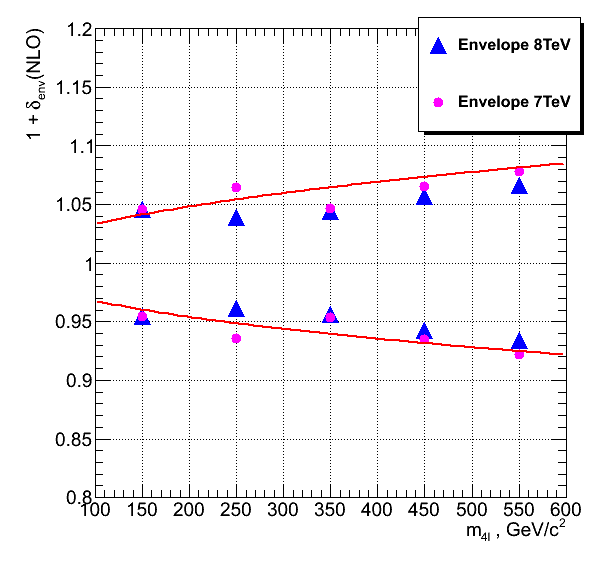
\includegraphics[width=0.48\textwidth,angle=0]{Chapters/Chapter4/Systematics/NLOZZ_pdf.png}
   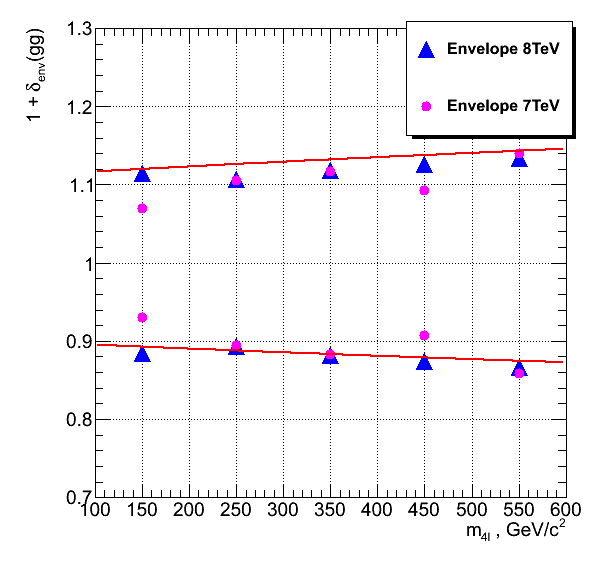
\includegraphics[width=0.48\textwidth,angle=0]{Chapters/Chapter4/Systematics/ggZZ_pdf.png}
   \caption{ PDF$+\alpha_s$ uncertainties for (left) $pp \to ZZ \to
     4\ell$ at NLO and (right) $gg \to ZZ \to 4\ell$ processes.  The
     points are evaluated uncertainties. The curves are the fit
     systematic error $\kappa(m_{4\ell})$ to be used in the
     statistical analysis.  These errors are driven by two independent
     nuisance parameters \textit{pdf\_qqbar} for $pp \to ZZ \to 4\ell$
     at NLO and \textit{pdf\_gg} for $gg \to ZZ \to 4\ell$.
    \label{fig:ZZ_PDFErrors}}
\end{center}
\end{figure}
\begin{figure}
 \begin{center}
   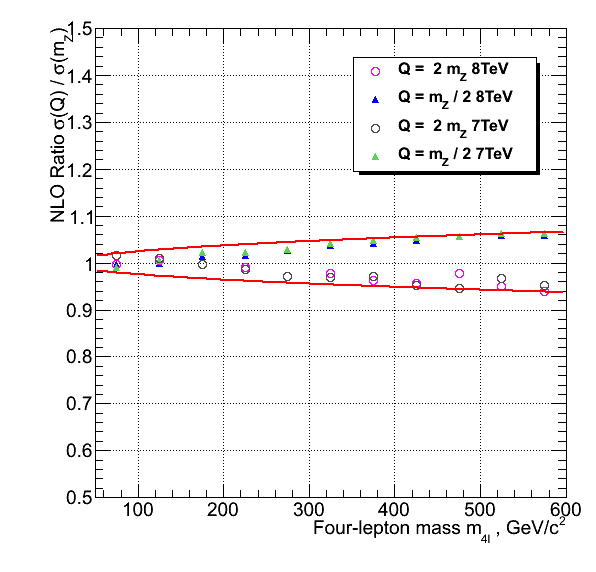
\includegraphics[width=0.48\textwidth,angle=0]{Chapters/Chapter4/Systematics/NLOZZ_QCD_Scale.png}
   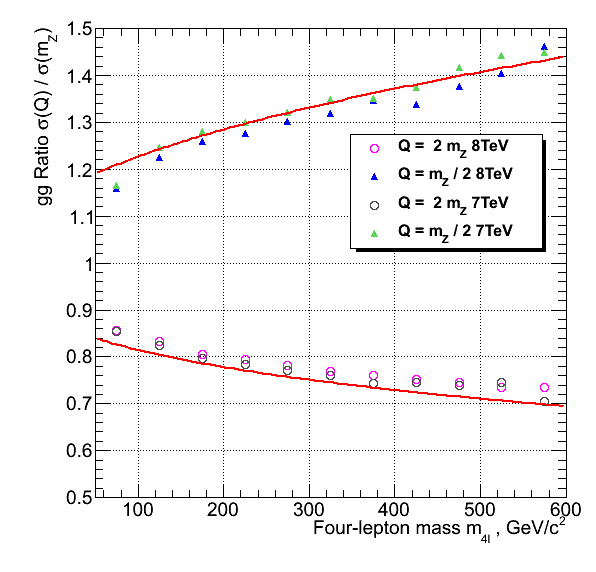
\includegraphics[width=0.48\textwidth,angle=0]{Chapters/Chapter4/Systematics/ggZZ_QCD_Scale.png}
   \caption{ QCD scale uncertainties for (left) $pp \to ZZ \to 4\ell$
     at NLO and (right) $gg \to ZZ \to 4\ell$ processes.  The points
     are evaluated uncertainties. The curves are the fit systematic
     error $\kappa(m_{4\ell})$ to be used in the statistical analysis.
     These errors are driven by two independent nuisance parameters
     \textit{QCDscale\_VV} for $pp \to ZZ \to 4\ell$ at NLO and
     \textit{QCDscale\_ggVV} for $gg \to ZZ \to 4\ell$.
    \label{fig:ZZ_QCDErrors}}
\end{center}
\end{figure}

\subsection{Uncertainties on the Reducible Background Predictions}

For the determination of the shape of the $m_{4 \ell}$ distribution for the channels where $Z_2 \to ee$, the two channels $4e$ and $2\mu2e$ are treated
together.  The uncertainty of the $m_{4\ell}$ shape is driven by that of the 3P1F component, of which the statistics is limited. To simplify the 
statistical analysis, the uncertainty of the $m_{4\ell}$ shape is included a global normalization uncertainty of $20\%$.
\par
For the determination of the shape of the $m_{4 \ell}$ distribution for the channels where $Z_2 \to \mu\mu$, the two channels $4\mu$ and $2e2\mu$ are
treated together. The shape is rather well constrained, and any uncertainty on the $m_{4 \ell}$ distribution is absorbed in the large systematic
uncertainty of $40\%$ set on the event yields.
\par
The channels $2e2\mu$ (where the $Z_1$ is made from two electrons) and $2\mu 2e$ (where the $Z_1$ is made from two muons) are treated together. 
The mass shape used for this channel is the average of the two shapes presented above, weighted by the event yields expected in the two channels, 
and a global normalization uncertainty of $25 \%$ is used.

\subsection{Uncertainties on Signal Shape and Yields}

The uncertainties affecting the shape of the signal arise from the non perfect knowledge of the lepton scale and resolution, which originates from 
the dependency of the scale and resolution on $p_{\rm T}$, $\eta$ and from run conditions. For muons, the energy scale uncertainty is less than
0.1\%, which propagates to about 0.1\% on the $4\ell$ mass for $4\mu$ events. For electrons, the systematics due to the energy scale dependency
on $p_{\rm T}$ are 0.3\% systematic for $4e$ final state and extra 0.2\% systematic for $2e2\mu$ final state on the mean of the double-sided Crystal
Ball function. In addition, the uncertainty on the resolution is estimated to be $20\%$.
\par
For both integrated and differential cross sections measurements, the uncertainty on the signal yields comes from uncertainties
on the luminosity
and imperfect knowledge on single lepton efficiency which are taken from ~\cite{Chatrchyan:2013mxa, Aad:2013xqa}. For the "wrong" signal process, its mass
spectrum is taken from $WH, ZH, t\bar{t}H$ MC samples and parameterized using a Landau function. The mean and sigma of the Landau function are allowed to
float to cover the difference in the shape between $WH, ZH, t\bar{t}H$ processes. The expected normalization on the "wrong" signal process is taken from
SM prediction, i.e., the sum of contributions from $WH, ZH, t\bar{t}H$ processes. We allow this normalization varies according to a log-uniform
distribution, of which the 1-$\sigma$ variation corresponds to enhance or suppress the expected normalization by one order of magnitude.

\subsection{Uncertainties on Jet Energy Scale}

For differential cross section measurement as a function jet multiplicity, the uncertainty due to jet energy scale has non-negligible effect which can effect 
the number of reco jet distribution while has no impact on number of gen jet distribution. Figure \ref{fig:jesvsjer} shows the number of 
reco-jet distribution variation when the reco jet energy is scaled up by 1-$\sigma$. As a result, the efficiency of events with number $N_{gen-jet}$ gen
jets being reconstructed as events with $N_{reco-jet}$ reco jets will vary according to the variation of the jet energy scale. To correlate the variation
due to reco-jet energy scale for signal and background events in different reco bin, we introduce a nuisance parameter $\theta_{JES}$ with unit Gaussian
distribution,
\begin{equation}
\mathrm{eff}(N_{reco-jet}, N_{gen-jet} | \theta_{JES}) = (1+\lambda(N_{reco-jet}, N_{gen-jet} )\theta_{JES})\times\mathrm{eff}(N_{reco-jet}, N_{gen-jet} | \theta_{JES}=0).
\end{equation}

If define $\theta_{JES}=\pm 1$ corresponding to 1-$\sigma$ variation of the reco-jet energy scale, then the parameter $\lambda(N_{reco-jet})$ can be
calculated using the nominal efficiency and efficiency at 1-$\sigma$ variation of the reco-jet energy scale as
\begin{eqnarray}
&&\lambda(N_{reco-jet}, N_{gen-jet} )\nonumber\\
&=& \frac{\mathrm{eff}(N_{reco-jet}, N_{gen-jet} | \theta_{JES}=\pm 1)-\mathrm{eff}(N_{reco-jet}, N_{gen-jet} | \theta_{JES}=0)}{\mathrm{eff}(N_{reco-jet}, N_{gen-jet} | \theta_{JES}=0)}
\end{eqnarray}

In practice, $\lambda(N_{reco-jet}, N_{gen-jet})$ is calculated using MC samples or control region data for each reco bin for both signal and background
processes. Examples of  $\lambda(N_{reco-jet}, N_{gen-jet})$ factors can be seen in Table~\ref{tab:jesSM}.
\begin{table}[!h!tb]
\begin{center}
\small
\caption{
Percent change in events when increasing the jet energy scale by 1$\sigma$ for various signal model (all final states combined).
\label{tab:jesSM}
}
\begin{tabular}{|l|c|c|c|c|} \hline
Sample & N(jets)=0 & N(jets)=1 & N(jets)=2 & N(jets)$\geq$3 \\ \hline
gg$\rightarrow$H ({\sc powheg+JHUgen}) 125 $\GeV$ & -0.027 & 0.024 & 0.075 & 0.104 \\
gg$\rightarrow$H ({\sc minloHJJ}) 125 $\GeV$ & -0.023 & 0.028 & 0.073 & 0.120 \\
VBF ({\sc powheg}) 125 $\GeV$ & -0.088 & -0.028 & 0.025 & 0.081 \\
WH ({\sc pythia}) 125 $\GeV$ & -0.050 & -0.028 & 0.029 & 0.097 \\
ZH ({\sc pythia}) 125 $\GeV$ & -0.032 & -0.034 & 0.032 & 0.071 \\
ttH ({\sc pythia})125 $\GeV$ & 0.000 & -0.157 & -0.053 & 0.010 \\
\hline
\end{tabular}
\normalsize
\end{center}
\end{table}
%%%%%5
 \subsection{Uncertainties on the Pileup Jet ID Efficiency and the Jet Energy Resolution}

The uncertainties on the jet ID efficiency also contribute to the uncertainties on the jet counting (i.e., applying or not applying the jet ID cut 
should change the unfolding matrix).
The Pileup Jet ID efficiency measured in data agrees with simulation very well in all regions except for $|\eta|>3.0$, as studied in 
Ref. \cite{Aad:pile_up_jet_ID}.
Following those Pileup Jet ID efficiency studies, we have applied the correction factors for jets with $|\eta|>3.0$ in three bins of $p_{T}$: factor
0.90 for 30$<p_{T}<$36, factor 0.94 for 36$<p_{T}<$50, and factor 0.97 for $p_{T}>$50. The remaining uncertainty on the jet ID efficiency is then small
compared to the JES uncertainty and can be neglected.
\par
In addition, we have also checked if the uncertainties on the jet energy resolution (JER) contribute to the uncertainties on the jet multiplicity
measurement. We have estimated the JER uncertainties according to Jet/MET recommendation, and we have found that the uncertainty due to JER is much smaller 
than (and covered by) the JES uncertainty. For this reason, the JER uncertainty is not added separately. Comparisons of the JER uncertainty and
JES uncertainty for different production modes is shown in Figure~\ref{fig:jesvsjer} in Appendix~\ref{app:JetSystematics}.

\subsection{Uncertainty Due to Model Dependence}

One of the major goals of this analysis is to provide the model-independent measurements of $\Hllll$ integrated and differential
cross sections. To achieve a high degree of the model independence, we introduced isolation in the definition of the fiducial phase space and excluded
the "wrong" signal contributions from the fiducial phase space the definition. However, there is unavoidable remaining model dependence both in the 
integrated and differential cross section measurements. The efficiency for integrated cross section measurement is consistent between different models 
with about 10\% uncertainty, and this uncertainty can be up to 25\% in case of the number of jet differential cross section measurements. In addition, the 
non-fiducial signal also contributes to model dependence. A graphical representation of the model
dependence of this ratio is shows in the Figure~\ref{fig:modeldep-inclusive}.
\par
To properly include the correlations of all the sources of the model dependence, we extract the systematic uncertainty due to signal model dependence
in the following way: for each signal model, we use the corresponding MC sample to extract the fiducial signal efficiencies, non-fiducial signal fraction, 
and $\lambda(N_{reco-jet}, N_{gen-jet} )$ in case of the number of jets differential measurement. The integrated and differential 
cross section results are extracted with these inputs generated according to the SM composition of the Higgs boson production modes. We then extract
the results using the inputs of individual models which correspond to each of the Higgs production mechanisms in proton-proton collisions, rare $\Hllll$ decay 
through virtual photon(s) and exotic spin/parity models. The largest difference between the results of these individual measurements
and the result corresponding to the SM-like prediction we quote as the systematic uncertainty associated with the model dependence.
\begin{figure}[!h!tb]
  \begin{center}
      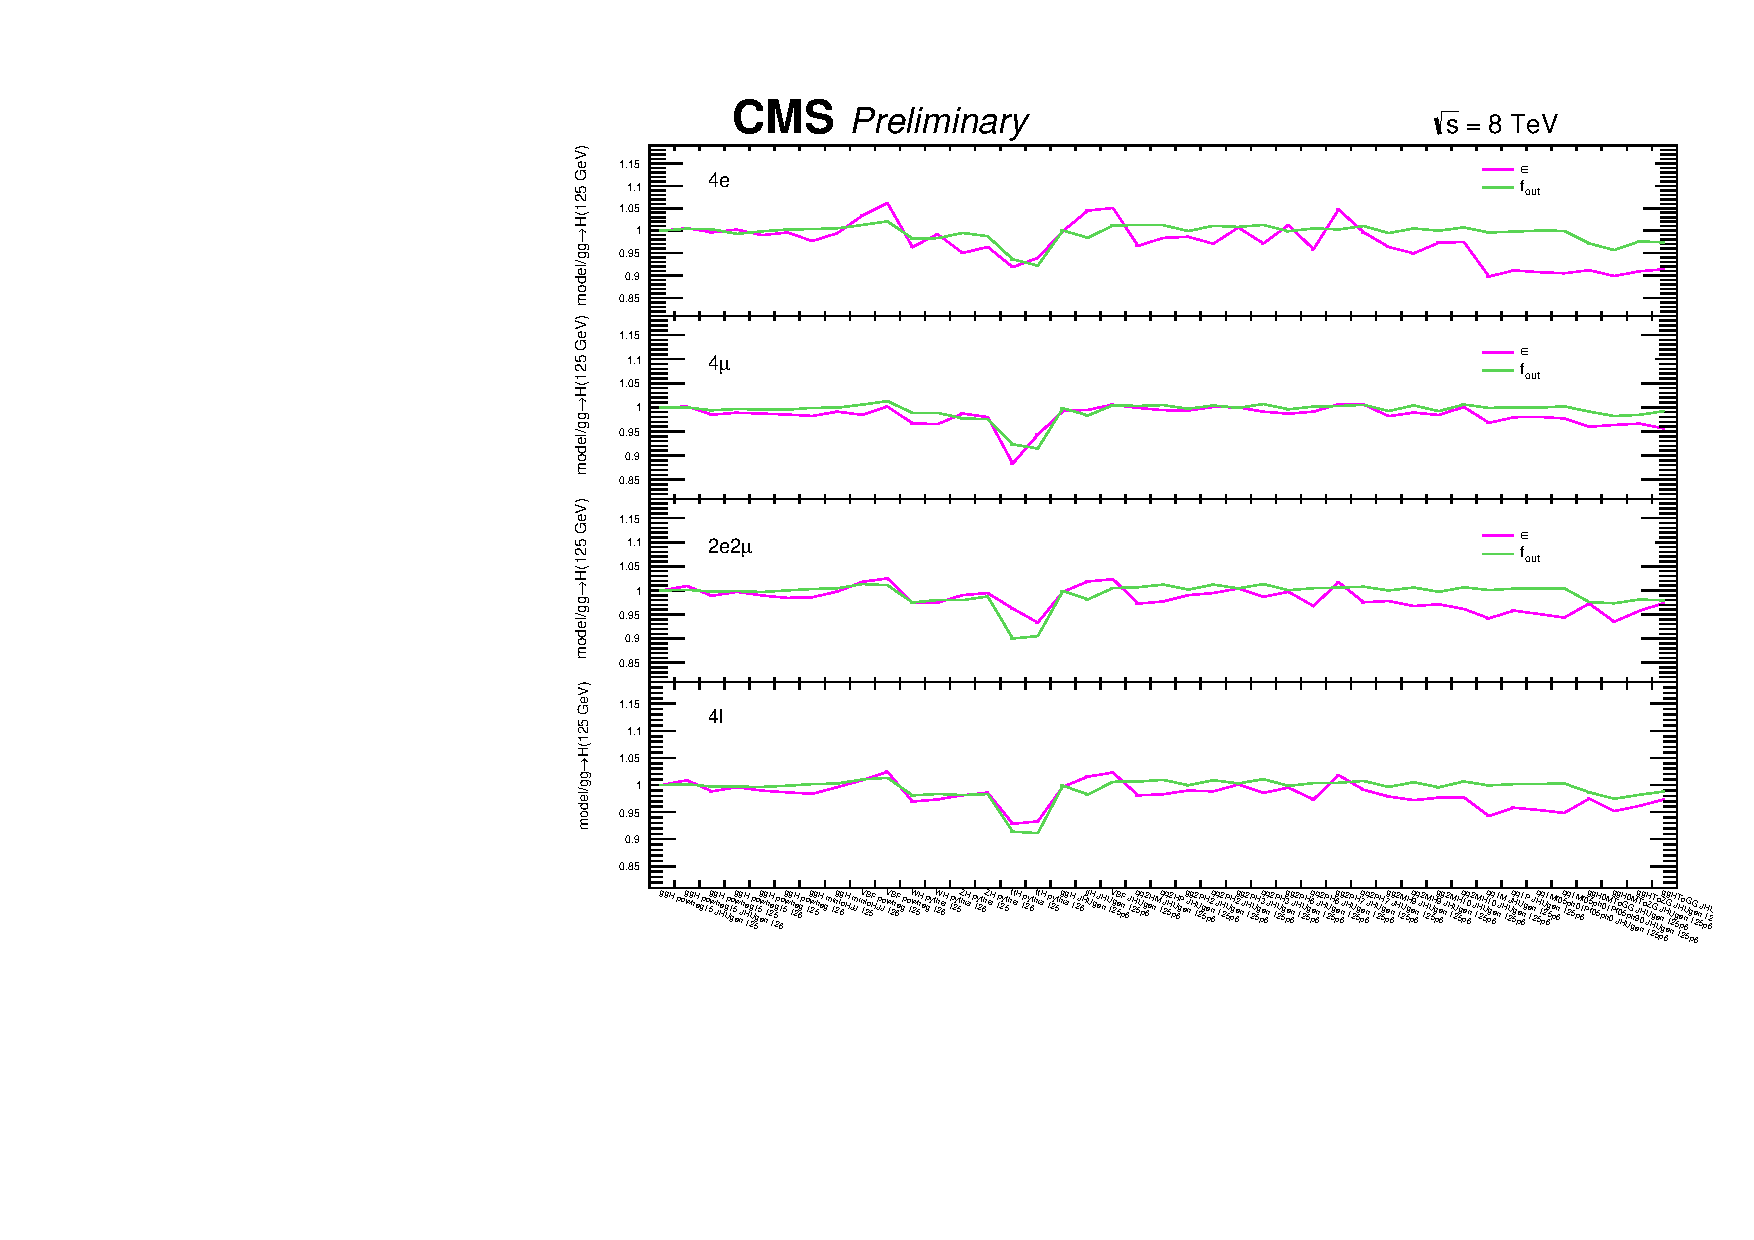
\includegraphics[width=0.95\textwidth,angle=0]{Plots/modeldep_inclusive.pdf}
    \caption{Ratio of integrated $\epsilon$ and $f_{\rm nonfid}$ for all signal models to the integrated $\epsilon$ and $f_{\rm nonfid}$ from the gg$\rightarrow$H production mode ({\sc powheg+JHUgen} 125 $\GeV$).}
  \label{fig:modeldep-inclusive}
  \end{center}
\end{figure}
\par
Additionally, we asses the model dependence uncertainty by taking into account the experimental constraints from the exiting CMS measurements. We
consider the Higgs boson to be a SM-like spin-zero boson with SM-like production mechanisms (all exotic decays and spin-parity models excluded), and
we allow the cross-section for the individual production mechanisms to vary within ranges that correspond to the allowed 95\% CL intervals from the
latest CMS combined results on the Higgs boson properties. In this case, the systematic uncertainty associated with the model dependence is 3-5\% in
case of the number of jets differential measurements, and it is smaller than 1\% for all the other measurements. The results can be found in
Appendix~\ref{app:restrictive_md}.
\par
As a test of the method, we also generate an alternative Asimov dataset according to a model which consists purely of ZH production and with
a cross section set to the total SM cross section. We then unfold this dataset using the the nominal SM values for the efficiencies and out
of acceptance fractions. The results of this test are shown in Appendix~\ref{app:alternateasimov}.
\par
The imprecision in the cross section measurements due to the $m_{H}$ being fixed in the fit procedure is estimated from simulation to be ~2\% per
0.6 GeV shift in mass. As the uncertainty on the CMS mass measurements is 0.3~GeV, the additional systematic uncertainty on the cross section measurement
would correspond of 1\%, and is covered by the larger already existing systematic uncertainties.
The Summary of all systematic uncertainties affecting $\Hllll$ cross section measurements is tabulated in Table~\ref{tab:SystOverview_runI}.

\begin{table}
\centering
\caption{
 Summary of all systematic uncertainties affecting $\Hllll$  cross section measurements.
\label{tab:SystOverview_runI}
}
\begin{tabular}{lc}
\hline
\multicolumn{2}{c}{Summary of relative systematic uncertainties} \\
\hline
\multicolumn{2}{c}{}  \\[-0.35cm]
\multicolumn{2}{c}{Common experimental uncertainties} \\
\hline
Luminosity & 2.2\% (7\TeV), 2.6\% (8\TeV) \\
Lepton identification/reconstruction efficiencies & \phantom{0}4--10\% \\
\hline
\multicolumn{2}{c}{}  \\[-0.35cm]
\multicolumn{2}{c}{Background related uncertainties} \\
\hline
QCD scale ($\Pq\Paq\to\Z\Z$, $\Pg\Pg\to\Z\Z$) & \phantom{0}3--24\% \\
PDF set ($\Pq\Paq\to\Z\Z$, $\Pg\Pg\to\Z\Z$) & 3--7\% \\
Reducible background ($\Z+\mathrm{X}$) & 20--40\% \\
Jet resolution and energy scale & \phantom{0}2--16\% \\
\hline
\multicolumn{2}{c}{}  \\[-0.35cm]
\multicolumn{2}{c}{Signal related uncertainties} \\
\hline
Lepton energy scale & 0.1--0.3\% \\
Lepton energy resolution & 20\% \\
Jet energy scale and resolution & \phantom{0}3--12\% \\
\hline
\multicolumn{2}{c}{}  \\[-0.35cm]
\multicolumn{2}{c}{Combinatorial signal-induced contribution} \\
\hline
Effect on the final measurement & \phantom{0}4--11\% \\
\hline
\multicolumn{2}{c}{}  \\[-0.35cm]
\multicolumn{2}{c}{Model dependence} \\
\hline
With exp. constraints on prod. modes \& exotic models & 1--5\% \\
No exp. constraints on prod. modes \& exotic models & \phantom{0}7--25\% \\
\hline
\end{tabular}
\normalsize
\end{table}


